% ===================================================================
\chapter{Results}
\label{ch:results}

This chapter follows the two stages of Section~\ref{sec:stages}. It first
reports the screening of all eight methods. It then breaks down where the
compression of the two selected algorithms comes from, and finally reports how
they were checked and how they performed on the FPGA board.

% -------------------------------------------------------------------
\section{Stage 1: screening eight methods}
\label{sec:stage1}

All eight methods were run on the same 50 ColoRadar frames, using all 16
receive channels. The reference chain found \num{9934} detections in these
frames. Table~\ref{tab:stage1} and Figure~\ref{fig:stage1} give the results.

\begin{table}[htbp]
\centering
\caption[Stage 1: the eight methods]{Stage 1: all eight methods, 50-frame
average, 16 receive channels. ``Missed'' is the false negative rate, FDR is the
false discovery rate (Section~\ref{sec:metrics}) and NF is the noise floor.
DRHE and LPC predict at lag $\nTx$ and use the original dictionary.}
\label{tab:stage1}
\small
\begin{tabular}{l|l|c|c|c|c|c}
\textbf{Method} & \textbf{Type} & \textbf{CR} & \textbf{Missed (\%)} & \textbf{FDR (\%)} & \textbf{NF (dBFS)} & \textbf{SNR (dB)}\\
\hline
FP16       & reference & 1.00 & 0.00  & 0.00 & $-105.64$ & 35.50\\
FX16       & reference & 1.00 & 3.77  & 1.11 & $-105.37$ & 35.36\\
BAQ        & lossy     & 3.76 & 10.44 & 9.69 & $-105.08$ & 35.08\\
RDVLE      & lossy     & 1.12 & 24.01 & 4.62 & $-102.27$ & 33.17\\
RDVLE+UDRE & lossy     & 2.56 & 28.73 & 4.44 & $-101.78$ & 33.00\\
DRHE fp16  & lossless\textsuperscript{*} & 1.04 & 0.05 & 0.01 & $-105.64$ & 35.51\\
\textbf{DRHE} & lossless & \textbf{3.75} & 3.77 & 1.11 & $-105.37$ & 35.36\\
\textbf{LPC}  & lossless & \textbf{3.70} & 3.77 & 1.11 & $-105.37$ & 35.36\\
\multicolumn{7}{@{}l}{\footnotesize\textsuperscript{*}lossless with respect to its FP16 input, which is itself rounded from the reference.}
\end{tabular}
\end{table}

\begin{figure}[htbp]
\centering
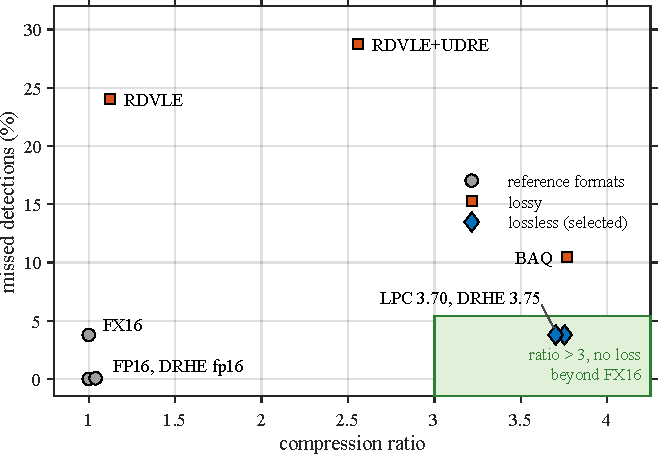
\includegraphics[width=0.8\textwidth]{fig_stage1.pdf}
\caption[Compression against missed detections]{Compression ratio against
missed detections for the eight methods. Better methods sit further to the
right, as they make the data smaller, and lower down, as they miss fewer
detections. Only DRHE and LPC reach the shaded region, which has a ratio above
three and no loss beyond FX16. The lossy methods pay for their ratio in missed
detections, and storing the data as floating point barely compresses it.}
\label{fig:stage1}
\end{figure}

FX16, DRHE and LPC have the same detection results, because both coders give
back the FX16 codes bit for bit. These rows therefore show the cost of the
quantisation step alone. It misses \SI{3.77}{\percent} of the detections and
adds \SI{1.11}{\percent} false ones, and none of this is caused by
compression. BAQ reaches \num{3.76}, which is the same ratio as DRHE. However,
it misses \SI{10.44}{\percent} of the reference detections, and
\SI{9.69}{\percent} of its detections are false. This is nearly three times
the miss rate and nine times the false discovery rate, with no gain in ratio.
RDVLE and RDVLE+UDRE are worse on both counts. DRHE applied to FP16 values
almost removes the quantisation loss, but it only compresses by \num{1.04}.
This is because a half-precision value keeps fine noise detail at every size,
so the compressor's input needs to be integers. DRHE (\num{3.75}) and LPC
(\num{3.70}) are the only methods that compress by more than three without
adding a missed detection. Both are above the 2.8 that three cascades need on
one Gigabit link (Section~\ref{sec:linkreq}), so both were taken forward.

\subsection{The cost of the quantisation step}
\label{sec:quant}

FX16 causes all of the detection loss in the lossless methods.
Table~\ref{tab:quant} therefore compares four ways of producing the 16-bit
codes. The standard fixed scaling only uses \SI{1.33}{\percent} of the
\texttt{int16} range. Scaling each frame to its own peak reduces the
quantisation error by a factor of 67, and the companding curve of Deng and
Huang \cite{deng2024} reduces it even further.

\begin{table}[htbp]
\centering
\caption[Quantisation study]{Four ways of producing the 16-bit codes, ColoRadar
frame 0, all 16 receive channels. ``relRMS'' is the RMS error of the range-FFT
values relative to their RMS. ``RD error'' is the RMS error of the
range--Doppler map in dB. ``int16 use'' is the largest code as a fraction of
\num{32767}. The last column is the lossless DRHE ratio on the resulting codes.}
\label{tab:quant}
\small
\setlength{\tabcolsep}{3pt}
\begin{tabular}{l|c|c|c|c|c}
\textbf{Quantiser} & \textbf{relRMS (\%)} & \textbf{PSNR (dB)} & \textbf{RD error (dB)} & \textbf{int16 use (\%)} & \textbf{DRHE CR}\\
\hline
FP16 (reference)            & 0.0205 & 101.97 & 0.0049 & ---   & ---\\
FX16, fixed scaling         & 1.8636 & 64.44  & 0.4336 & 1.33  & \textbf{3.80}\\
FX16, scaled to frame peak  & 0.0278 & 101.09 & 0.0054 & 89.20 & 1.18\\
FX16, companded \cite{deng2024} & 0.0048 & 114.38 & 0.0011 & 94.28 & 0.78\\
\end{tabular}
\end{table}

However, the compression ratio moves the other way. When the range is filled,
lossless DRHE only compresses by \num{1.18}, and with companding it makes the
data larger. The fixed scaling leaves about six of the sixteen bits as copies
of the sign bit. Filling the range turns these bits into fine detail, which is
mostly receiver noise that a lossless coder has to keep. Hence, the
quantisation error can only be removed by giving up almost all of the
compression. The fixed scaling was therefore kept, as in Kiem's design.

% -------------------------------------------------------------------
\section{Stage 2: the prediction lag}
\label{sec:predaxisres}

Stage~2 uses the four-receiver frames that the hardware processes.
Table~\ref{tab:predaxis} compares each predictor with the no-prediction
baseline, at lag 1 and at lag $\nTx$.

\begin{table}[htbp]
\centering
\caption[The prediction lag]{Compression ratio against the no-prediction
baseline, 50 frames, four receive channels, original dictionary, 256-bit
padding. The predictor rows are from HLS C-simulation, and all are lossless.}
\label{tab:predaxis}
\small
\begin{tabular}{l|c|c}
\textbf{Configuration} & \textbf{CR} & \textbf{vs.\ no prediction}\\
\hline
No prediction (Huffman coding only)            & \num{3.479} & ---\\
DRHE, lag 1 (adjacent ramp)                    & \num{3.310} & $-4.9\,\%$\\
LPC, lags 1, 2                                 & \num{3.385} & $-2.7\,\%$\\
\textbf{DRHE, lag $\nTx$}                      & \textbf{\num{3.751}} & $\mathbf{+7.8\,\%}$\\
\textbf{LPC, lags $\nTx$, $2\nTx$}             & \textbf{\num{3.697}} & $\mathbf{+6.3\,\%}$\\
\end{tabular}
\end{table}

On this radar the adjacent ramp comes from another transmitter. Predicting from
it is worse than not predicting at all, for both algorithms. Predicting from
the same transmitter turns a \SI{4.9}{\percent} loss into a
\SI{7.8}{\percent} gain for DRHE, and a \SI{2.7}{\percent} loss into a
\SI{6.3}{\percent} gain for LPC. The largest residuals also shrink. The 99th
percentile of the residual size falls from \num{80.6} with no prediction to
\num{15.8} for DRHE and \num{8.2} for LPC. LPC loses less than DRHE at lag 1.
When there is little correlation, the Yule--Walker solution pushes LPC's
coefficients towards zero, which is the same as not predicting. The median
$a_1$ is $-0.02$ at lag 1, compared with $0.40$ at lag $\nTx$. DRHE's
coefficients are fixed, so it keeps following a phase trend that is not there.
Everything from here on uses lag $\nTx$.

% -------------------------------------------------------------------
\section{Where the compression comes from}
\label{sec:decomp}

Both algorithms use the same entropy coder, so their ratio can be built up in
three steps (Table~\ref{tab:decomp} and Figure~\ref{fig:crbars}). The first
step is the coder on the FX16 codes alone. The second is what prediction adds,
and the third is what a dictionary built for the prediction errors adds.

\begin{table}[htbp]
\centering
\caption[Where the compression comes from]{The compression ratio built up step
by step, 50 frames, four receive channels (MATLAB). The ``held out'' column is
the total on frames 5 to 49 only, which the re-derived dictionary was not
trained on.}
\label{tab:decomp}
\small
\begin{tabular}{l|c|c|c|c|c}
& \textbf{Huffman coding} & \textbf{+ prediction} & \textbf{+ re-derived} & \textbf{Total} & \textbf{Total,}\\
& \textbf{only} & & \textbf{dictionary} & & \textbf{held out}\\
\hline
DRHE & \num{3.479} & $+\num{0.272}$ & $+\num{0.466}$ & \textbf{\num{4.218}} & \num{4.207}\\
LPC  & \num{3.479} & $+\num{0.218}$ & $+\num{0.707}$ & \textbf{\num{4.404}} & \num{4.372}\\
\end{tabular}
\end{table}

\begin{figure}[htbp]
\centering
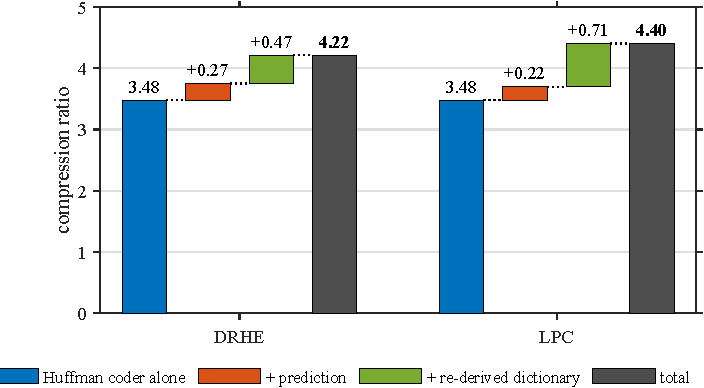
\includegraphics[width=0.8\textwidth]{fig_cr_bars.pdf}
\caption[Compression ratio, step by step]{The compression ratio built up step by
step. Huffman coding alone reaches \num{3.48}, and prediction adds \num{0.22}
to \num{0.27}. For both algorithms, the re-derived dictionary adds more than
prediction does.}
\label{fig:crbars}
\end{figure}

Most of the ratio comes before any prediction. The entropy coder alone reaches
\num{3.48}. This is mainly because the top bits of each FX16 code are unused,
and because most of a range-FFT frame is close to zero
(Section~\ref{sec:ratiomeaning}). Prediction adds \SIrange{6}{8}{\percent},
and the re-derived dictionary adds more than prediction does.

% -------------------------------------------------------------------
\section{The re-derived dictionary}
\label{sec:dictresult}

The original dictionary gives its shortest codes to categories 2 to 4.
However, most prediction errors fall in categories 0 to 2
(Table~\ref{tab:dictshare}). The re-derived dictionary gives these three
categories codes of three, two and one bits. For DRHE, the average codeword
then falls from \num{2.70} to \num{2.24} bits per value. For LPC it falls
from \num{2.80} to \num{2.12}.

\begin{table}[htbp]
\centering
\caption[What the re-derived dictionary changes]{Share of DRHE's prediction
errors by size $S_4$, and the codeword length each dictionary gives it (50
frames, four receive channels). Bold marks the three most common sizes.}
\label{tab:dictshare}
\small
\begin{tabular}{l|c|c|c|c|c|c|c}
\textbf{Size $S_4$} & \textbf{0} & \textbf{1} & \textbf{2} & \textbf{3} & \textbf{4} & \textbf{5} & \textbf{Average code}\\
\hline
Share of errors (\%)      & \textbf{17.6} & \textbf{30.9} & \textbf{34.1} & 13.8 & 2.5 & 0.6 & ---\\
Code length, original     & 4 & 3 & 2 & 2 & 2 & 5 & \num{2.70} bits\\
Code length, re-derived   & \textbf{3} & \textbf{2} & \textbf{1} & 4 & 5 & 6 & \textbf{\num{2.24} bits}\\
\end{tabular}
\end{table}

The dictionaries were trained on frames 0 to 4. On the 45 frames they did not
see, they reach \num{4.207} for DRHE and \num{4.372} for LPC. This is within
\SI{1}{\percent} of their results over all 50 frames. The FPGA cores give
exactly the same ratios as MATLAB, \num{4.21704} and \num{4.40345}. The new
dictionaries also change which algorithm compresses better. DRHE leads by
\SI{1.5}{\percent} with the original dictionary, but LPC leads by
\SI{4.4}{\percent} when each has its own dictionary. LPC's errors were always
the smaller of the two. However, the original dictionary cannot code anything in
fewer than four bits, which hid the difference.

% -------------------------------------------------------------------
\section{Frame-to-frame variation}
\label{sec:perframe}

\begin{figure}[htbp]
\centering
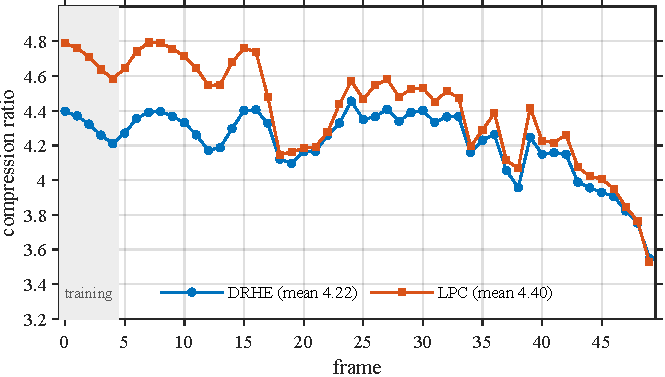
\includegraphics[width=0.8\textwidth]{fig_cr_frames.pdf}
\caption[Compression ratio of each frame]{Compression ratio of each of the 50
frames, with the re-derived dictionaries. Frames 0 to 4 (shaded) were used to
train the dictionaries, and the other 45 were not. LPC is ahead on almost every
frame, and both algorithms change with the scene in the same way.}
\label{fig:crframes}
\end{figure}

The ratio varies from about \num{3.5} to \num{4.8} across the recording, and
the two algorithms rise and fall together (Figure~\ref{fig:crframes}). Frames
with more strong returns have larger prediction errors, so they compress less.
A link has to be sized for the worst frame, and a ratio of \num{3.5} still
leaves a wide margin.

% -------------------------------------------------------------------
\section{Verification}
\label{sec:verifres}

Every level of the ladder in Section~\ref{sec:ladder} passed with no
difference between input and output ($\mathrm{MaxDiff} = 0$):

\begin{itemize}
\item \textbf{C-simulation}, 50 frames (\num{157286400} input bits per
design). Both compressors, with both dictionaries, give back every sample
exactly. The bit counts match MATLAB on every frame once the padding of the
last 256-bit word is counted.
\item \textbf{RTL co-simulation} and all eight \textbf{edge cases}
(Table~\ref{tab:edgecases}) pass for both algorithms. Random input grows by
\SI{67}{\percent}, which any lossless coder must do on data that cannot be
compressed.
\item \textbf{Board, compressors}. With both dictionaries, the compressed
output is byte for byte the same as the C-simulation on all 50 frames. The mean
ratios are \num{4.21704} for DRHE and \num{4.40345} for LPC with the
re-derived dictionaries, and \num{3.7508} and \num{3.6968} with the original
dictionary.
\item \textbf{Board, decoders}. The hardware decoders rebuild all 50 frames
exactly, word for word.
\item \textbf{Board, from raw ADC samples}. With the range FFT also on the
FPGA, the FX16 codes match its C-simulation, and the compressed streams match
the compressors' C-simulation. The decoders again rebuild every frame exactly.
\end{itemize}

\noindent
Every hardware compression ratio in this thesis is therefore a measured value.
Every stage, from raw ADC samples to rebuilt data, has also been run on the
FPGA.

% -------------------------------------------------------------------
\section{Speed and latency on the board}
\label{sec:boardtiming}

\begin{table}[htbp]
\centering
\caption[Measured timing on the board]{Timing measured on the KCU116 at
\SI{100}{\mega\hertz}, 50 frames of \SI{393216}{\byte}. Latency is from the last
input word read to the last output word written (Section~\ref{sec:metrics}).
For the decompressor, it is from the last compressed word read to the last
rebuilt word written. The compressor values are from the run with the original
dictionary. With the re-derived dictionaries they differ by at most 13 cycles.}
\label{tab:timing}
\small
\begin{tabular}{l|c|c}
& \textbf{DRHE} & \textbf{LPC}\\
\hline
Clock cycles per frame          & \num{61472}   & \num{325366}\\
Time per frame                  & \textbf{\SI{0.61}{\milli\second}} & \SI{3.25}{\milli\second}\\
Frames per second               & \num{1627}    & \num{307}\\
Input throughput                & \textbf{\SI{5.12}{Gbit/s}} & \SI{0.97}{Gbit/s}\\
End-to-end latency              & \textbf{\SI{13.1}{\micro\second}} & \SI{3006}{\micro\second}\\
\quad as a share of the frame time & \SI{2}{\percent} & \SI{92}{\percent}\\
\hline
Decompressor cycles per frame   & \num{196881}  & \lpcDecCycles\\
Decompression time per frame    & \SI{1.97}{\milli\second} & \lpcDecTime\\
Decompressor latency            & \SI{339}{\micro\second} & \lpcDecLat\\
\end{tabular}
\end{table}

\begin{figure}[htbp]
\centering
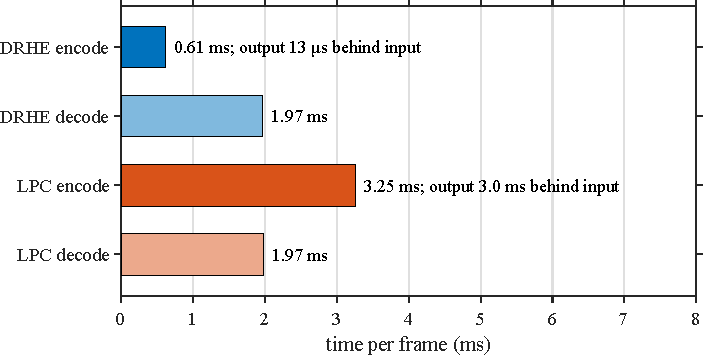
\includegraphics[width=0.8\textwidth]{fig_timing.pdf}
\caption[Time per frame on the FPGA]{Time to encode and decode one frame on the
FPGA, measured on the board in the same runs as Table~\ref{tab:timing}, with
each encoder's output delay. DRHE sends its output as the data arrives, but
LPC must wait for the whole frame before it can send anything. Both decoders
decode one value per clock.}
\label{fig:timing}
\end{figure}

DRHE works as a stream (Table~\ref{tab:timing} and Figure~\ref{fig:timing}).
Its time per frame of \SI{0.61}{\milli\second} is two clocks per input word
($\mathrm{II} = 2$), plus a short pipeline fill on each ramp. Its last
compressed word leaves \SI{13.1}{\micro\second} after the last raw word
arrives. LPC takes \SI{3.25}{\milli\second}, and \SI{3.0}{\milli\second} of
this comes after the last input word. This is because its coefficients cannot
be calculated until every ramp has arrived. It is 230 times DRHE's latency, and
no change in scheduling can remove it as long as the coefficients are fitted to
the frame being compressed. Both decoders run at almost exactly one value per
clock, taking \SI{1.97}{\milli\second} each, whatever the data. Their
latencies are the work still left when the compressed input ends. All of these
are fast compared with ColoRadar's \SI{200}{\milli\second} frame period.
DRHE's compressor uses \SI{0.3}{\percent} of it, LPC's uses under
\SI{2}{\percent}, and each decoder uses about \SI{1}{\percent}.

% -------------------------------------------------------------------
\section{Chip resources}
\label{sec:resources}

\begin{table}[htbp]
\centering
\caption[Resources per core]{Post-route resources of each core on the
\texttt{XCKU5P} (\num{216960} LUT, \num{433920} FF, 480 BRAM, \num{1824} DSP).
BRAM is in 36\,Kb blocks.}
\label{tab:resources}
\small
\begin{tabular}{l|l|c|c|c|c}
& & \textbf{LUT} & \textbf{FF} & \textbf{BRAM} & \textbf{DSP}\\
\hline
DRHE & compressor   & \num{35444} & \num{23528} & 40   & 132\\
     & decompressor & \num{14155} & \num{9245}  & 32.5 & 46\\
     & \textbf{both} & \textbf{\num{49599}} (\SI{23}{\percent}) & \num{32773} & 72.5 & 178\\
\hline
LPC  & compressor   & \num{33820} & \num{20083} & 108  & 158\\
     & decompressor & \num{15212} & \num{7207}  & 0    & 23\\
     & \textbf{both} & \textbf{\num{49032}} (\SI{23}{\percent}) & \num{27290} & 108 & 181\\
\end{tabular}
\end{table}

\begin{figure}[htbp]
\centering
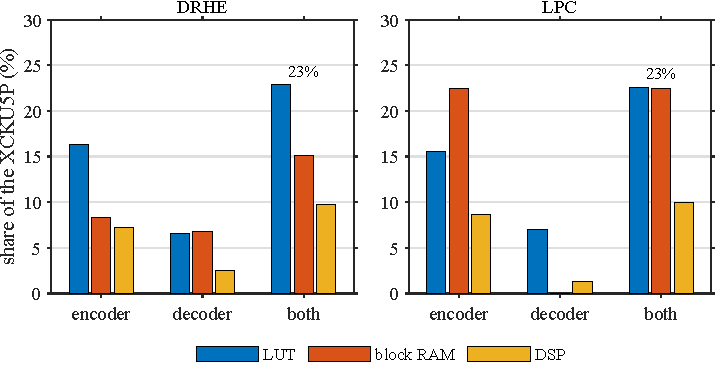
\includegraphics[width=0.8\textwidth]{fig_resources.pdf}
\caption[FPGA resources]{Share of the \texttt{XCKU5P}'s LUTs, block RAMs and
DSP slices used by each core after routing in the board system. The bars show
the compressor, the decompressor, and both together.}
\label{fig:resources}
\end{figure}

For both algorithms, the encoder and decoder together use under a quarter of
the chip's logic (Table~\ref{tab:resources} and Figure~\ref{fig:resources}).
The whole test system uses \SI{38}{\percent} for DRHE and \SI{37}{\percent}
for LPC. The two compressors use almost the same logic, but they differ in
memory. LPC needs 108 block RAMs, 96 of them for its frame buffer, while DRHE
needs 40 for its stored values. The decoders are the other way round. The LPC
decoder receives its coefficients in the bitstream, so it needs no block RAM.
Power was not measured on the board. With default switching activity, Vivado
estimates \HW{drhen}{ptotal}\,W for the DRHE compressor core and
\HW{lpcn}{ptotal}\,W for the LPC one. About \HW{drhen}{pstatic}\,W of this is
static power. The rest, the dynamic power, works out to \HW{drhen}{pJbit} and
\HW{lpcn}{pJbit}\,pJ per input bit.

% -------------------------------------------------------------------
\section{Starting from raw ADC samples}
\label{sec:feresults}

With the range FFT on the chip (Section~\ref{sec:fehw}), the board takes the
raw ADC samples of each frame and does everything else itself
(Table~\ref{tab:fe}).

\begin{table}[htbp]
\centering
\caption[Measured with the range FFT on chip]{Board measurements, 50 frames,
with the FX16 codes from MATLAB (as in the rest of this chapter) and from the
range FFT on the FPGA. The input rate is in FX16 codes for the first and in raw
ADC samples for the second. Latency is from the last input word read to the
last compressed word written.}
\label{tab:fe}
\small
\begin{tabular}{l|c|c|c|c}
& \multicolumn{2}{c|}{\textbf{DRHE}} & \multicolumn{2}{c}{\textbf{LPC}}\\
\cline{2-3}\cline{4-5}
\textbf{FFT in} & \textbf{MATLAB} & \textbf{FPGA} & \textbf{MATLAB} & \textbf{FPGA}\\
\hline
Compression ratio     & \num{4.21704} & \num{4.21696} & \num{4.40345} & \num{4.40338}\\
Cycles per frame      & \num{61472}   & \num{75626}   & \num{325366}  & \num{375957}\\
Time per frame        & \SI{0.61}{\milli\second} & \SI{0.76}{\milli\second} & \SI{3.25}{\milli\second} & \SI{3.76}{\milli\second}\\
Input rate            & \SI{5.12}{Gbit/s} & \SI{8.32}{Gbit/s} & \SI{0.97}{Gbit/s} & \SI{1.67}{Gbit/s}\\
End-to-end latency    & \SI{13.1}{\micro\second} & \SI{21.3}{\micro\second} & \SI{3006}{\micro\second} & \SI{3024}{\micro\second}\\
\end{tabular}
\end{table}

Out of \num{9830400} codes, \num{1522} (\SI{0.016}{\percent}) differ from
MATLAB's, each by one step. These are values that lie almost exactly on a
rounding boundary. The ratios only change in the fifth significant figure. Both
sets of codes have exactly the $1/\sqrt{12}$\,LSB RMS error of ideal rounding,
and their detections differ by three out of \num{11148}
(Table~\ref{tab:fedet}). Hence, MATLAB's range FFT gives the same results as
the hardware would. With the front end added, it now sets the speed. DRHE takes
\SI{0.76}{\milli\second} per frame, which is still \SI{8.3}{Gbit/s} of raw
ADC data, and LPC's \SI{3.0}{\milli\second} after the last input word does
not change. The front end uses \SI{7}{\percent} of the LUTs and 296 DSPs. The
whole system then uses \SI{47}{\percent} of the LUTs for DRHE and
\SI{46}{\percent} for LPC.

\begin{table}[htbp]
\centering
\caption[Detection loss with the range FFT on chip]{Detections of the two
sets of FX16 codes against the double-precision reference, 50 frames, four
receive channels (\num{11148} reference detections). FP\% is a false discovery
rate (Section~\ref{sec:detectionmetrics}).}
\label{tab:fedet}
\small
\begin{tabular}{l|c|c|c|c|c}
\textbf{Codes} & \textbf{FN (\%)} & \textbf{FP (\%)} & \textbf{NF (dBFS)} & \textbf{SNR (dB)} & \textbf{error (LSB RMS)}\\
\hline
Reference (double)  & ---  & ---  & $-106.06$ & 36.56 & ---\\
FX16, MATLAB        & 4.19 & 1.81 & $-105.81$ & 36.40 & 0.2887\\
FX16, FPGA          & 4.17 & 1.80 & $-105.81$ & 36.40 & 0.2887\\
\end{tabular}
\end{table}

% -------------------------------------------------------------------
\section{The two algorithms side by side}
\label{sec:headtohead}

\begin{table}[htbp]
\centering
\caption[DRHE and LPC compared]{DRHE and LPC compared on every measured
quantity. Bold marks the better of the two on each row.}
\label{tab:headtohead}
\small
\begin{tabular}{l|c|c}
& \textbf{DRHE} & \textbf{LPC}\\
\hline
Lossless on the board (50 frames, both dictionaries) & yes & yes\\
Compression ratio, original dictionary (board)    & \textbf{\num{3.75}} & \num{3.70}\\
Compression ratio, re-derived dictionary (board)  & \num{4.22} & \textbf{\num{4.40}}\\
Time per frame                                   & \textbf{\SI{0.61}{\milli\second}} & \SI{3.25}{\milli\second}\\
End-to-end latency                               & \textbf{\SI{13.1}{\micro\second}} & \SI{3006}{\micro\second}\\
First output available                           & \textbf{immediately} & after the whole frame\\
Decompression time per frame                     & \SI{1.97}{\milli\second} & \lpcDecTime\\
Compressor frame buffer                          & \textbf{none} & \SI{3.0}{\mebi bit}\\
Encoder + decoder LUTs                           & \SI{23}{\percent} & \SI{23}{\percent}\\
Encoder + decoder BRAM (36\,Kb blocks)          & \textbf{72.5} & 108\\
Side information                                 & \textbf{none} & \SI{1.04}{\percent}\\
\end{tabular}
\end{table}

Table~\ref{tab:headtohead} brings the results together. The two algorithms are
close on compression ratio, and which one leads depends on the dictionary. They
use about the same logic, and their decoders run at the same speed. DRHE is
ahead on time, latency and memory. It compresses a frame five times faster,
does not need a frame buffer, and its output lags its input by microseconds
rather than milliseconds.
